% $Header: /cvsroot/latex-beamer/latex-beamer/solutions/conference-talks/conference-ornate-20min.en.tex,v 1.7 2007/01/28 20:48:23 tantau Exp $

\documentclass{beamer}

% This file is a solution template for:

% - Talk at a conference/colloquium.
% - Talk length is about 20min.
% - Style is ornate.



% Copyright 2004 by Till Tantau <tantau@users.sourceforge.net>.
%
% In principle, this file can be redistributed and/or modified under
% the terms of the GNU Public License, version 2.
%
% However, this file is supposed to be a template to be modified
% for your own needs. For this reason, if you use this file as a
% template and not specifically distribute it as part of a another
% package/program, I grant the extra permission to freely copy and
% modify this file as you see fit and even to delete this copyright
% notice. 


\mode<presentation>
{
  \usetheme{Warsaw}
  \usecolortheme{default}
  % or ...

  \setbeamercovered{transparent}
  % or whatever (possibly just delete it)
}

\usepackage{wrapfig}
\usepackage{tikz}
\usepackage{amsmath}

\newcommand{\bpm}{\begin{pmatrix}}
\newcommand{\epm}{\end{pmatrix}}

\usepackage[english]{babel}
% or whatever

\usepackage[latin1]{inputenc}
% or whatever

\usepackage{times}
\usepackage[T1]{fontenc}
% Or whatever. Note that the encoding and the font should match. If T1
% does not look nice, try deleting the line with the fontenc.


\title[Systematic MPC Constraint Handling] % (optional, use only with long paper titles)
{Systematic Model Predictive Controller Constraint Handling}

\subtitle
{Rigorous Geometric Methods}

\author[Campher, Sandrock] % (optional, use only with lots of authors)
{AH.~Campher \and C.~Sandrock}
% - Give the names in the same order as the appear in the paper.
% - Use the \inst{?} command only if the authors have different
%   affiliation.

\institute[University of Pretoria] % (optional, but mostly needed)
{ Department of Chemical Engineering\\
  University of Pretoria}
% - Use the \inst command only if there are several affiliations.
% - Keep it simple, no one is interested in your street address.

\date[SPSS 2010] % (optional, should be abbreviation of conference name)
{SAIChE Postgraduate Student Symposium, 2010}
% - Either use conference name or its abbreviation.
% - Not really informative to the audience, more for people (including
%   yourself) who are reading the slides online

\subject{Control Engineering}
% This is only inserted into the PDF information catalog. Can be left
% out. 

% Delete this, if you do not want the table of contents to pop up at
% the beginning of each subsection:
% \AtBeginSubsection[]
% {
%   \begin{frame}<beamer>{Outline}
%     \tableofcontents[currentsection,current subsection]
%   \end{frame}
% }


% If you wish to uncover everything in a step-wise fashion, uncomment
% the following command: 

%\beamerdefaultoverlayspecification{<+->}


\begin{document}

\begin{frame}
  \titlepage
\end{frame}

%\begin{frame}{Outline}
%  \tableofcontents
%  % You might wish to add the option [pausesections]
%\end{frame}

\section{Background}

\subsection{Model Predictive Control}

\begin{frame}{Model Predictive Control}
One of the most popular algorithms for advanced control.
\begin{wrapfigure}{r}{72mm}
  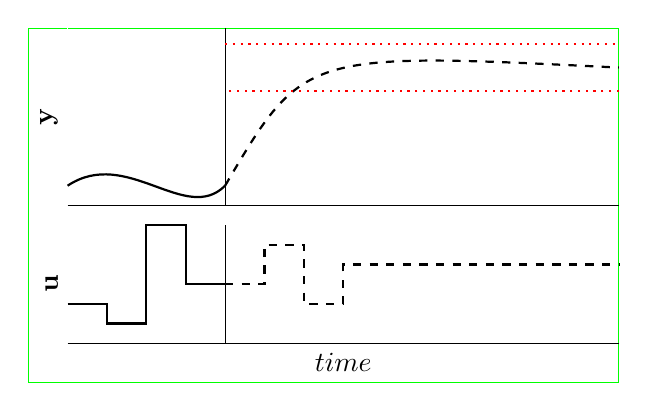
\begin{tikzpicture}[scale=1,stream/.style={->,thick}]
    %myborder
    \draw [color=green] (0,0) rectangle (7.5,4.5);
    %mpcoutputs
    \draw (0.5,0.5+1.75) -- coordinate (x axis mid) (7.5,0.5+1.75);
    \draw [color=white] (0.5,0.5+1.75) -- coordinate (y axis mid) (0.5,4.5);
    \node[rotate=90, above] at (y axis mid) {$\bf y$};
    \draw (2.5,0.5+1.75) -- (2.5,4.5);

    \draw [thick] (0.5,2.5) .. controls (1.25,3) and (2,2) .. (2.5,2.5);
    \draw [thick,dashed] (2.5,2.5) .. controls (3.5,4.2) .. (7.5,4);
    \draw [thick,dotted,color=red] (2.5,4.3) -- (7.5,4.3) (7.5,3.7) -- (2.5,3.7);


    %mpcinputs
    \draw (0.5,0.5) -- coordinate (x axis mid) (7.5,0.5);
    \draw [color=white] (0.5,0.5) -- coordinate (y axis mid) (0.5,2);
    \node[below] at (x axis mid) {$time$};
    \node[rotate=90, above] at (y axis mid) {$\bf u$};
    \draw (2.5,0.5) -- (2.5,2);

    \draw [thick] (0.5,1) -- (1,1) -- (1,0.75) -- (1.5,0.75) -- (1.5,2) -- (2,2)-- (2,1.25) -- (2.5,1.25);
    \draw [thick,dashed] (2.5,1.25) -- (3,1.25) -- (3,1.75) -- (3.5,1.75) -- (3.5,1) -- (4,1)-- (4,1.5) -- (7.5,1.5);

  \end{tikzpicture}
\end{wrapfigure}\\
Selling points;
  \begin{itemize}
    \item
      Predictions
    \item
      Constraints
    \item
      Commercial MPC software
  \end{itemize}
\vfill
\end{frame}

\begin{frame}{The Working of MPC}
MPC is essentially a 4 step process;
\begin{wrapfigure}{r}{72mm}
  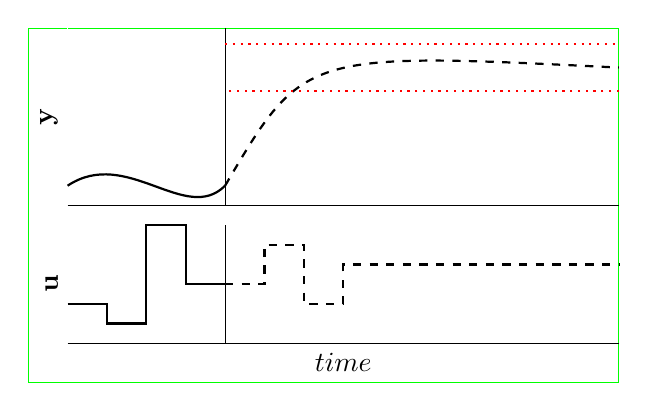
\begin{tikzpicture}[scale=1,stream/.style={->,thick}]
    %myborder
    \draw [color=green] (0,0) rectangle (7.5,4.5);
    %mpcoutputs
    \draw (0.5,0.5+1.75) -- coordinate (x axis mid) (7.5,0.5+1.75);
    \draw [color=white] (0.5,0.5+1.75) -- coordinate (y axis mid) (0.5,4.5);
    \node[rotate=90, above] at (y axis mid) {$\bf y$};
    \draw (2.5,0.5+1.75) -- (2.5,4.5);

    \draw [thick] (0.5,2.5) .. controls (1.25,3) and (2,2) .. (2.5,2.5);
    \draw [thick,dashed] (2.5,2.5) .. controls (3.5,4.2) .. (7.5,4);
    \draw [thick,dotted,color=red] (2.5,4.3) -- (7.5,4.3) (7.5,3.7) -- (2.5,3.7);


    %mpcinputs
    \draw (0.5,0.5) -- coordinate (x axis mid) (7.5,0.5);
    \draw [color=white] (0.5,0.5) -- coordinate (y axis mid) (0.5,2);
    \node[below] at (x axis mid) {$time$};
    \node[rotate=90, above] at (y axis mid) {$\bf u$};
    \draw (2.5,0.5) -- (2.5,2);

    \draw [thick] (0.5,1) -- (1,1) -- (1,0.75) -- (1.5,0.75) -- (1.5,2) -- (2,2)-- (2,1.25) -- (2.5,1.25);
    \draw [thick,dashed] (2.5,1.25) -- (3,1.25) -- (3,1.75) -- (3.5,1.75) -- (3.5,1) -- (4,1)-- (4,1.5) -- (7.5,1.5);

  \end{tikzpicture}
\end{wrapfigure}
  \begin{enumerate}
    \item
      Measure
    \item
      Predict
    \item
      Optimize / Calculate
    \item
      Apply
  \end{enumerate}
\vfill
\end{frame}


\subsection{Previous Work}

\begin{frame}{Process Models, Inputs, Outputs and Constraints}
\begin{center}
  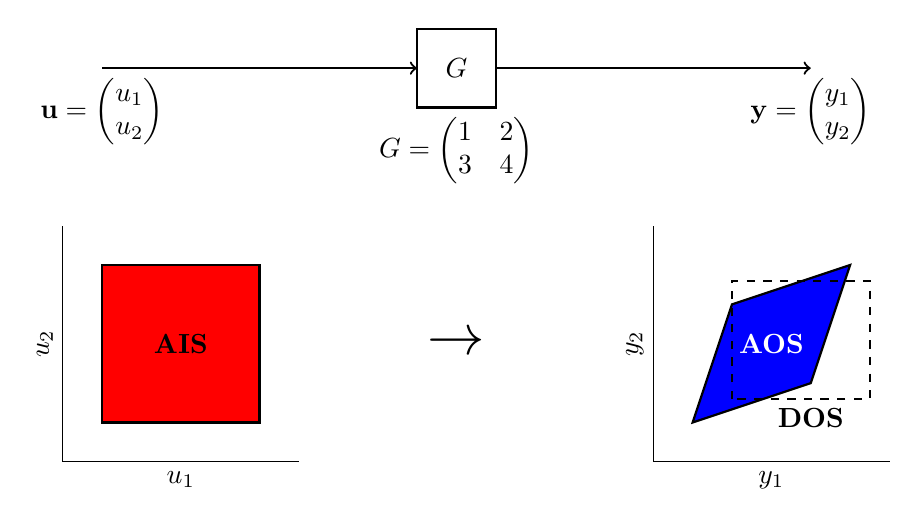
\begin{tikzpicture}[scale=1,stream/.style={->,thick}]
    %model
    \draw [thick] (-0.5,-0.5) rectangle (0.5,0.5);
    \node at (0,0){$G$};
    \node [below] at (0,-0.5){$G=\begin{pmatrix}
                                        1 & 2 \\
                                        3 & 4 \\
                                 \end{pmatrix}$};
    %inputs
    \draw [stream] (-4.5,0) -- node[below,at start]{${\bf u}=\bpm u_1 \\ u_2\epm$}
                          (-0.5,0);
    %outputs
    \draw [stream] (0.5,0) -- node[below,at end]{${\bf y}=\bpm y_1 \\ y_2 \epm$}
                          (4.5,0);
    %AIS
    \draw (-5,-5) -- coordinate (x axis mid) (-2,-5);
    \draw (-5,-5) -- coordinate (y axis mid) (-5,-2);
    \node[below] at (x axis mid) {$u_1$};
    \node[rotate=90, above] at (y axis mid) {$u_2$};
    \draw [thick,fill=red] (-4.5,-4.5) rectangle (-2.5,-2.5);
    \node at (-3.5,-3.5){\bf AIS};
    
    \node at (0,-3.5){\bf \huge $\to$};
    
    %AOS
    \draw (-5+7.5,-5) -- coordinate (x axis mid) (-2+7.5,-5);
    \draw (-5+7.5,-5) -- coordinate (y axis mid) (-5+7.5,-2);
    \node[below] at (x axis mid) {$y_1$};
    \node[rotate=90, above] at (y axis mid) {$y_2$};
    \draw [thick,fill=blue] (3,-4.5) -- (3.5,-3) -- (5,-2.5) -- (4.5,-4) -- cycle;
    \node [color=white] at (-3.5+7.5,-3.5){\bf AOS};
    
    % DOS
    \draw [thick,dashed] (3.5,-4-0.2) rectangle (5.25,-2.5-0.2);
    \node [below] at (4.5,-4.2){\bf DOS};

    %COS

  \end{tikzpicture}
\end{center}
\end{frame}

\begin{frame}{The Operability Index's Application to MPC}
\begin{wrapfigure}{r}{50mm}
  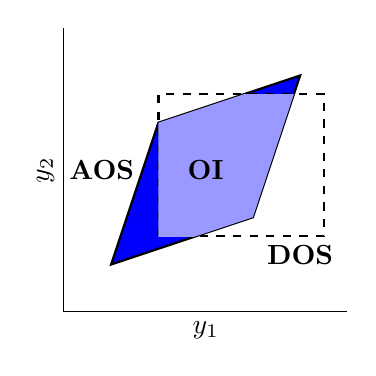
\begin{tikzpicture}[scale=1.2,stream/.style={->,thick}]
    %AOS
    \draw (-5+7.5,-5) -- coordinate (x axis mid) (-2+7.5,-5);
    \draw (-5+7.5,-5) -- coordinate (y axis mid) (-5+7.5,-2);
    \node[below] at (x axis mid) {$y_1$};
    \node[rotate=90, above] at (y axis mid) {$y_2$};
    \draw [thick,fill=blue] (3,-4.5) -- (3.5,-3) -- (5,-2.5) -- (4.5,-4) -- cycle;
    \node at (-4.6+7.5,-3.5){\bf AOS};
    
    % DOS
    \draw [thick,dashed] (3.5,-4-0.2) rectangle (5.25,-2.5-0.2);
    \node [below] at (5,-4.2){\bf DOS};

\begin{scope}
    \clip (3.5,-4-0.2) rectangle (5.25,-2.5-0.2);
    \clip (3,-4.5) -- (3.5,-3) -- (5,-2.5) -- (4.5,-4) -- cycle;
    \fill[color=blue!40] (-5+7.5,-5) rectangle (5.5,-2);
\end{scope}
    \node at (4,-3.5){\bf OI};
  \end{tikzpicture}
\end{wrapfigure}
Definition: 

  \begin{itemize}
    \item
      $OI = \frac{\mu(AOS \cap DOS)}{\mu(DOS)}$
    \item
      Bigger is better
  \end{itemize}
\vfill
\end{frame} 


\begin{frame}{Addition of Disturbances}
\begin{center}
  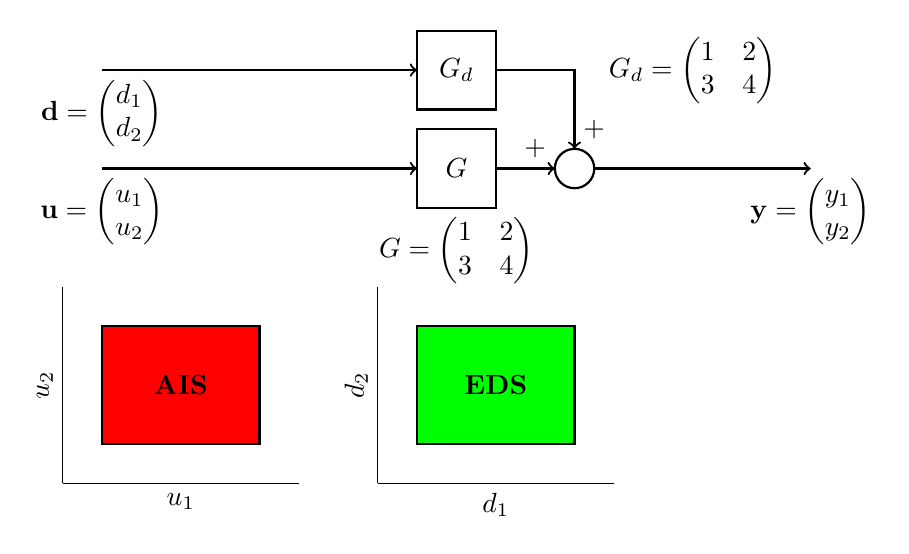
\begin{tikzpicture}[scale=1,stream/.style={->,thick}]
    %model
    \draw [thick] (-0.5,-0.5) rectangle (0.5,0.5);
    \node at (0,0){$G$};
    \node [below] at (0,-0.5){$G=\begin{pmatrix}
                                        1 & 2 \\
                                        3 & 4 \\
                                 \end{pmatrix}$};
    %d model
    \draw [thick] (-0.5,0.75) rectangle (0.5,1.75);
    \node at (0,1.25){$G_d$};
    \node at (3,1.25){$G_d=\begin{pmatrix}
                                        1 & 2 \\
                                        3 & 4 \\
                                 \end{pmatrix}$};
    %d
    \draw [stream] (-4.5,1.25) -- node[below,at start]{${\bf d}=\bpm d_1 \\ d_2\epm$} (-0.5,1.25);
    \draw [stream] (0.5,1.25) -| (1.5,0.25);
    %sum
    \draw [thick] (1.5,0) circle (0.25);
    \node at (1,0.25){+};
    \node at (1.75,0.5){+};
    % inputs
    \draw [stream] (-4.5,0) -- node[below,at start]{${\bf u}=\bpm u_1 \\ u_2\epm$}
                          (-0.5,0);
    %outputs
    \draw [stream] (0.5,0) -- (1.25,0);
    \draw [stream] (1.75,0) -- node[below,at end]{${\bf y}=\bpm y_1 \\ y_2 \epm$}
                          (4.5,0);
    %AIS
    \draw (-5,-4) -- coordinate (x axis mid) (-2,-4);
    \draw (-5,-4) -- coordinate (y axis mid) (-5,-1.5);
    \node[below] at (x axis mid) {$u_1$};
    \node[rotate=90, above] at (y axis mid) {$u_2$};
    \draw [thick,fill=red] (-4.5,-3.5) rectangle (-2.5,-2);
    \node at (-3.5,-2.75){\bf AIS};
    
    %DIS
    \draw (-5+4,-4) -- coordinate (x axis mid) (-2+4,-4);
    \draw (-5+4,-4) -- coordinate (y axis mid) (-5+4,-1.5);
    \node[below] at (x axis mid) {$d_1$};
    \node[rotate=90, above] at (y axis mid) {$d_2$};
    \draw [thick,fill=green] (-4.5+4,-3.5) rectangle (-2.5+4,-2);
    \node at (-3.5+4,-2.75){\bf EDS};

  \end{tikzpicture}
\end{center}
\end{frame}


\begin{frame}{Addition of Disturbances (cont.)}
\begin{center}
  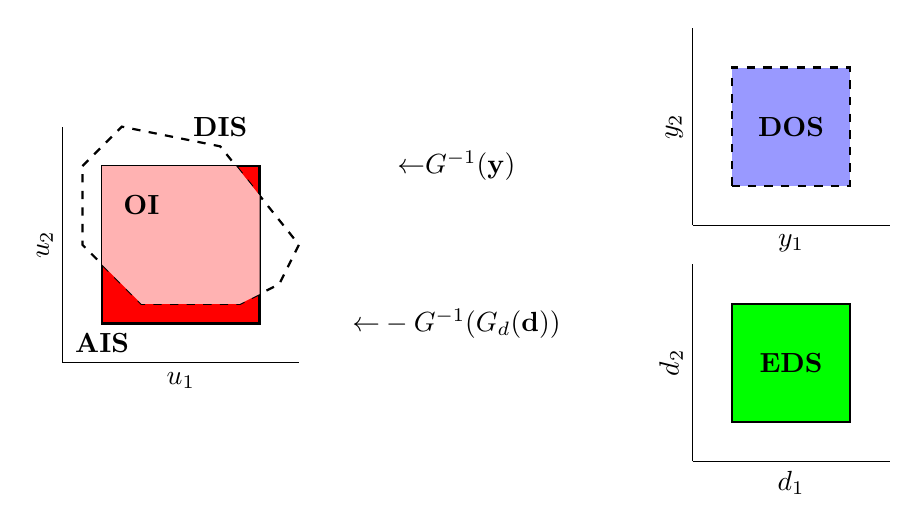
\begin{tikzpicture}[scale=1,stream/.style={->,thick}]
    %DOS
    \draw (3,0.25) -- coordinate (x axis mid) (5.5,0.25);
    \draw (3,0.25) -- coordinate (y axis mid) (3,2.75);
    \node[below] at (x axis mid) {$y_1$};
    \node[rotate=90, above] at (y axis mid) {$y_2$};
    \draw [thick,dashed,fill=blue!40] (3.5,0.75) rectangle (5,2.25);
    \node at (4.25,1.5){\bf DOS};
    
    %EDS
    \draw (3,-2.75) -- coordinate (x axis mid) (5.5,-2.75);
    \draw (3,-2.75) -- coordinate (y axis mid) (3,-0.25);
    \node[below] at (x axis mid) {$d_1$};
    \node[rotate=90, above] at (y axis mid) {$d_2$};
    \draw [thick,fill=green] (3.5,-2.25) rectangle (5,-0.75);
    \node at (4.25,-1.5){\bf EDS};
    
    %maps to
    \node at (0,1){${\huge \gets} G^{-1}({\bf y})$};
    \node at (0,-1){${\huge \gets} -G^{-1}(G_d({\bf d}))$};
    
    %AIS
    \draw (-5,-1.5) -- coordinate (x axis mid) (-2,-1.5);
    \draw (-5,-1.5) -- coordinate (y axis mid) (-5,1.5);
    \node[below] at (x axis mid) {$u_1$};
    \node[rotate=90, above] at (y axis mid) {$u_2$};
    \draw [thick,fill=red] (-4.5,-1) rectangle (-2.5,1);
    \node at (-4.5,-1.25){\bf AIS};

    %DIS
    \draw [thick,dashed] (-4.75,1) -- (-4.25,1.5) -- (-3,1.25) 
                         -- (-2,0) -- (-2.25,-0.5) -- (-2.75,-0.75) 
                         -- (-4,-0.75) -- (-4.75,0) -- cycle;
    \node at (-3,1.5){\bf DIS};

    \begin{scope}
    \clip (-4.5,-1) rectangle (-2.5,1);
    \clip (-4.75,1) -- (-4.25,1.5) -- (-3,1.25) 
                         -- (-2,0) -- (-2.25,-0.5) -- (-2.75,-0.75) 
                         -- (-4,-0.75) -- (-4.75,0) -- cycle;
    \fill[color=red!30] (-4.5,-1) rectangle (-2.5,1);
    \end{scope}    
    
    \node at (-4,0.5){\bf OI};

  \end{tikzpicture}
\end{center}
\end{frame}


\begin{frame}{Constraints and Their Application in MPC}
Commercial MPCs use constraints in;
  \begin{itemize}
    \item
      Control calculations
    \item
      Optimizers
      \begin{itemize}
        \item
          Static constraints
        \item
          Dynamic constraints
      \end{itemize}
  \end{itemize}
\end{frame}


\section{Method}

\subsection{Sample Problem}

\begin{frame}{The Sample Problem}
\begin{center}  
  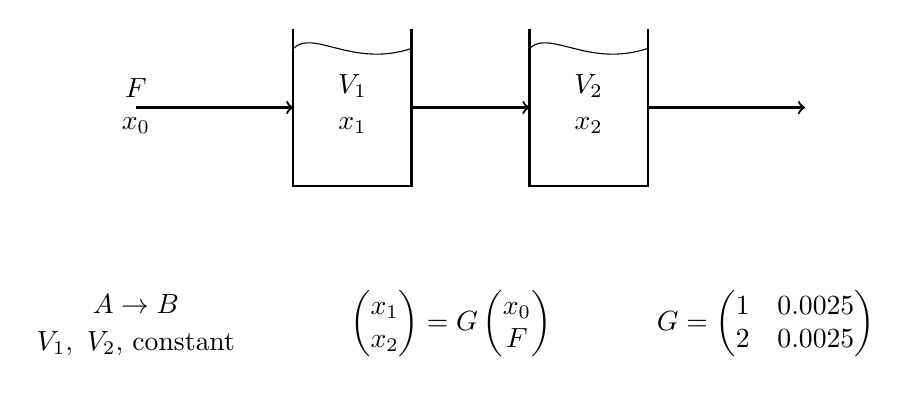
\begin{tikzpicture}[scale=1,stream/.style={->,thick}]
    \draw [thick] (0,2) -- (0,0) -- (1.5,0) -- (1.5,2);
    \draw [thick] (0+3,2) -- (0+3,0) -- (1.5+3,0) -- (1.5+3,2);
    \draw [stream] (-2,1) -- node [above,at start]{$F$} node [below, at start]{$x_0$} (0,1);
    \draw [stream] (1.5,1) -- (3,1);
    \draw [stream] (4.5,1) -- (6.5,1);
    \node [above] at (0.75,1){$V_1$}; \node [below] at (0.75,1){$x_1$};
    \node [above] at (0.75+3,1){$V_2$}; \node [below] at (0.75+3,1){$x_2$};
    \draw (0,1.75) .. controls (0.25,2) and (0.75,1.5) ..(1.5,1.75);
    \draw (3,1.75) .. controls (0.25+3,2) and (0.75+3,1.5) ..(4.5,1.75);
  
    \node at (-2,-1-1){$V_1,~V_2$, constant};
    \node at (-2,-0.5-1){$A \to B$};
    \node at (2,-0.75-1){$\bpm x_1\\x_2 \epm=G\bpm x_0 \\ F \epm$};
    \node at (6,-0.75-1){$G=\bpm 1 & 0.0025 \\
                               2 & 0.0025 \epm$};
  \end{tikzpicture}
\end{center}
\end{frame}

\begin{frame}{The Sample Problem (cont.)}
\begin{center}  
  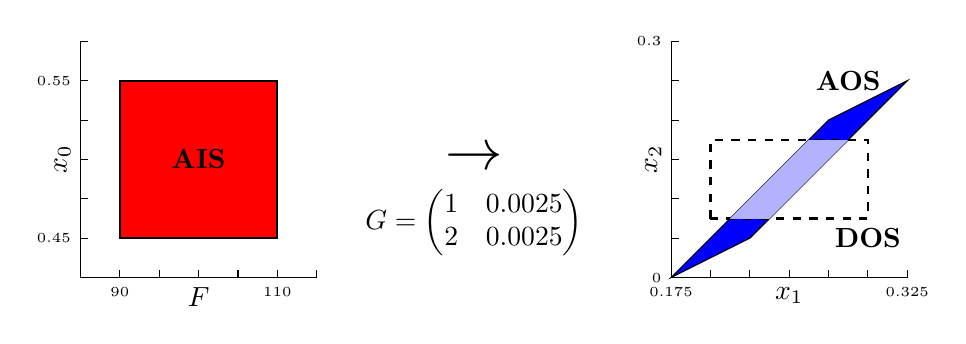
\begin{tikzpicture}[scale=1,stream/.style={->,thick}]
    %AIS
    \draw (0,0) -- coordinate (x axis mid) (3,0);
    \draw (0,0) -- coordinate (y axis mid) (0,3);
    \foreach \x in {0,0.5,...,3}
      \draw (\x,0) -- (\x,0.1);
    \foreach \y in {0,0.5,...,3}
      \draw (0,\y) -- (0.1,\y);
    \node[below] at (x axis mid) {$F$};
    \node[below] at (0.5,0) {\tiny 90};
    \node[below] at (2.5,0) {\tiny 110};
    \node[rotate=90, above] at (y axis mid) {$x_0$};
    \node[left] at (0,0.5) {\tiny 0.45};
    \node[left] at (0,2.5) {\tiny 0.55};
    \draw [thick,fill=red] (0.5,0.5) rectangle (2.5,2.5);
    \node at (1.5,1.5){\bf AIS};
    
    \node at (5,1.5){\bf \huge $\to$};
    \node [below] at (5,1.25){$G=\bpm 1 & 0.0025 \\
                               2 & 0.0025 \epm$};
    
    %AOS
    \def\mx{20}; \def\px{4};
    \def\my{10};
    \draw (7.5,0) -- coordinate (x axis mid) (3+7.5,0);
    \draw (7.5,0) -- coordinate (y axis mid) (7.5,3);
    \foreach \x in {7.5,8,...,10.5}
      \draw (\x,0) -- (\x,0.1);
    \foreach \y in {0,0.5,...,3}
      \draw (7.5,\y) -- (7.6,\y);
    \node[below] at (x axis mid) {$x_1$};
    \node[below] at (7.5,0) {\tiny 0.175};
    \node[below] at (10.5,0) {\tiny 0.325};
    \node[rotate=90, above] at (y axis mid) {$x_2$};
    \node[left] at (7.5,0) {\tiny 0};
    \node[left] at (7.5,3) {\tiny 0.3};
    \draw [fill=blue] (0.175*\mx + \px , 0) 
                         -- (0.225*\mx + \px,0.05*\my) 
                         -- (0.325*\mx + \px,0.25*\my) 
                         -- (0.275*\mx + \px,0.2*\my) -- cycle;
    \node at (9.75,2.5){\bf AOS};    
    % DOS  0.25 0.125
    \draw [thick,dashed] (0.2*\mx + \px,0.075*\my) rectangle
                         (0.3*\mx + \px,0.175*\my);
    \node at (10,0.5){\bf DOS};    

    \begin{scope}
    \clip (0.2*\mx + \px,0.075*\my) rectangle
                         (0.3*\mx + \px,0.175*\my);
    \clip (0.175*\mx + \px , 0) 
                         -- (0.225*\mx + \px,0.05*\my) 
                         -- (0.325*\mx + \px,0.25*\my) 
                         -- (0.275*\mx + \px,0.2*\my) -- cycle;
    \fill[color=blue!30] (0.2*\mx + \px,0.075*\my) rectangle
                         (0.3*\mx + \px,0.175*\my);
    \end{scope}    

  \end{tikzpicture}
\end{center}
\end{frame}


\subsection{Constraint Types}

\begin{frame}{A Combination of Constraint Types are Present}
Disambiguating the different types of constraints;
\begin{wrapfigure}{r}{35mm}
  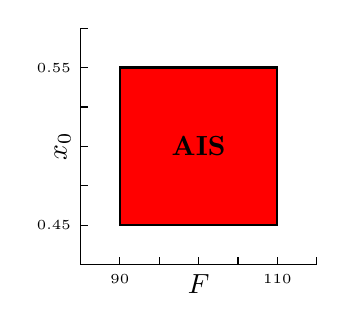
\begin{tikzpicture}[scale=1,stream/.style={->,thick}]
    %AIS
    \draw (0,0) -- coordinate (x axis mid) (3,0);
    \draw (0,0) -- coordinate (y axis mid) (0,3);
    \foreach \x in {0,0.5,...,3}
      \draw (\x,0) -- (\x,0.1);
    \foreach \y in {0,0.5,...,3}
      \draw (0,\y) -- (0.1,\y);
    \node[below] at (x axis mid) {$F$};
    \node[below] at (0.5,0) {\tiny 90};
    \node[below] at (2.5,0) {\tiny 110};
    \node[rotate=90, above] at (y axis mid) {$x_0$};
    \node[left] at (0,0.5) {\tiny 0.45};
    \node[left] at (0,2.5) {\tiny 0.55};
    \draw [thick,fill=red] (0.5,0.5) rectangle (2.5,2.5);
    \node at (1.5,1.5){\bf AIS};
  \end{tikzpicture}
\end{wrapfigure}

\begin{itemize}
  \item
    Operational constraints
    \begin{itemize}
      \item
        Control constraints
      \item
        Optimization constraints
    \end{itemize}
  \item
    Physical constraints
  \item
    Subspace construction \\ is ambiguous
\end{itemize}
\end{frame}


\subsection{Constraint Changes}

\begin{frame}{How Changing Constraints Affect Other Constraints}
Model dependency is clear, the exact effect isn't.
\vfill
Possible source of inconsistencies;
  \begin{itemize}
    \item
      DOS still in AOS?
    \item
      Decrease in operability
  \end{itemize}
\vfill
\end{frame}


\begin{frame}{Changing Constraints (cont.)}
\begin{center}  
  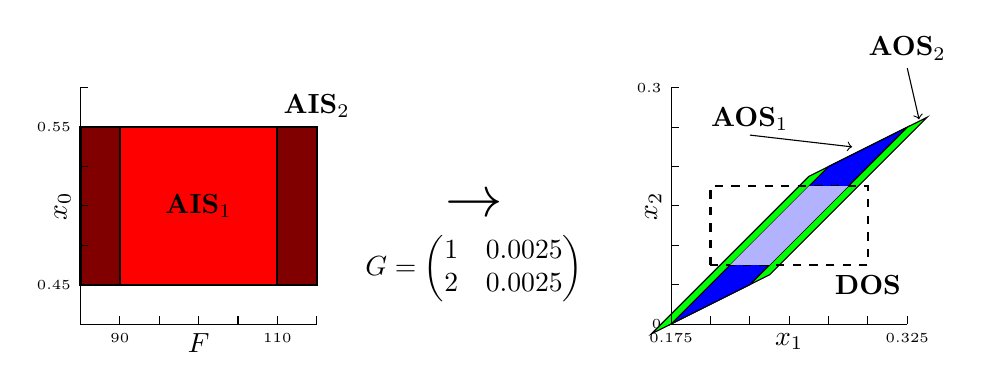
\begin{tikzpicture}[scale=1,stream/.style={->,thick}]
    %AIS
    \draw [thick,fill=red!50!black] (0,0.5) rectangle (3,2.5);
    \node [above] at (3,2.5){\bf AIS$_2$};
    \draw (0,0) -- coordinate (x axis mid) (3,0);
    \draw (0,0) -- coordinate (y axis mid) (0,3);
    \foreach \x in {0,0.5,...,3}
      \draw (\x,0) -- (\x,0.1);
    \foreach \y in {0,0.5,...,3}
      \draw (0,\y) -- (0.1,\y);
    \node[below] at (x axis mid) {$F$};
    \node[below] at (0.5,0) {\tiny 90};
    \node[below] at (2.5,0) {\tiny 110};
    \node[rotate=90, above] at (y axis mid) {$x_0$};
    \node[left] at (0,0.5) {\tiny 0.45};
    \node[left] at (0,2.5) {\tiny 0.55};
    \draw [thick,fill=red] (0.5,0.5) rectangle (2.5,2.5);
    \node at (1.5,1.5){\bf AIS$_1$};
    
    \node at (5,1.5){\bf \huge $\to$};
    \node [below] at (5,1.25){$G=\bpm 1 & 0.0025 \\
                               2 & 0.0025 \epm$};
    
    %AOS
    \def\mx{20}; \def\px{4};
    \def\my{10};

    \draw [fill=green]      (0.1625*\mx + \px,-0.0125*\my) 
                         -- (0.2375*\mx + \px, 0.0625*\my) 
                         -- (0.3375*\mx + \px, 0.2625*\my) 
                         -- (0.2625*\mx + \px, 0.1875*\my) -- cycle;
    \node at (10.5,3.5){\bf AOS$_2$};

    \draw [->] (8.5,2.4) -- (9.8,2.25);
    \draw [->] (10.5,3.25) -- (10.65,2.6);

    \draw (7.5,0) -- coordinate (x axis mid) (3+7.5,0);
    \draw (7.5,0) -- coordinate (y axis mid) (7.5,3);
    \foreach \x in {7.5,8,...,10.5}
      \draw (\x,0) -- (\x,0.1);
    \foreach \y in {0,0.5,...,3}
      \draw (7.5,\y) -- (7.6,\y);
    \node[below] at (x axis mid) {$x_1$};
    \node[below] at (7.5,0) {\tiny 0.175};
    \node[below] at (10.5,0) {\tiny 0.325};
    \node[rotate=90, above] at (y axis mid) {$x_2$};
    \node[left] at (7.5,0) {\tiny 0};
    \node[left] at (7.5,3) {\tiny 0.3};
    \draw [fill=blue] (0.175*\mx + \px , 0) 
                         -- (0.225*\mx + \px,0.05*\my) 
                         -- (0.325*\mx + \px,0.25*\my) 
                         -- (0.275*\mx + \px,0.2*\my) -- cycle;
    \node at (8.5,2.6){\bf AOS$_1$};    
    % DOS  0.25 0.125
    \draw [thick,dashed] (0.2*\mx + \px,0.075*\my) rectangle
                         (0.3*\mx + \px,0.175*\my);
    \node at (10,0.5){\bf DOS};    

    \begin{scope}
    \clip (0.2*\mx + \px,0.075*\my) rectangle
                         (0.3*\mx + \px,0.175*\my);
    \clip (0.175*\mx + \px , 0) 
                         -- (0.225*\mx + \px,0.05*\my) 
                         -- (0.325*\mx + \px,0.25*\my) 
                         -- (0.275*\mx + \px,0.2*\my) -- cycle;
    \fill[color=blue!30] (0.2*\mx + \px,0.075*\my) rectangle
                         (0.3*\mx + \px,0.175*\my);
    \end{scope}    

  \end{tikzpicture}
\end{center}
\end{frame}


\begin{frame}{Changing Constraints (cont.)}
\begin{center}  
  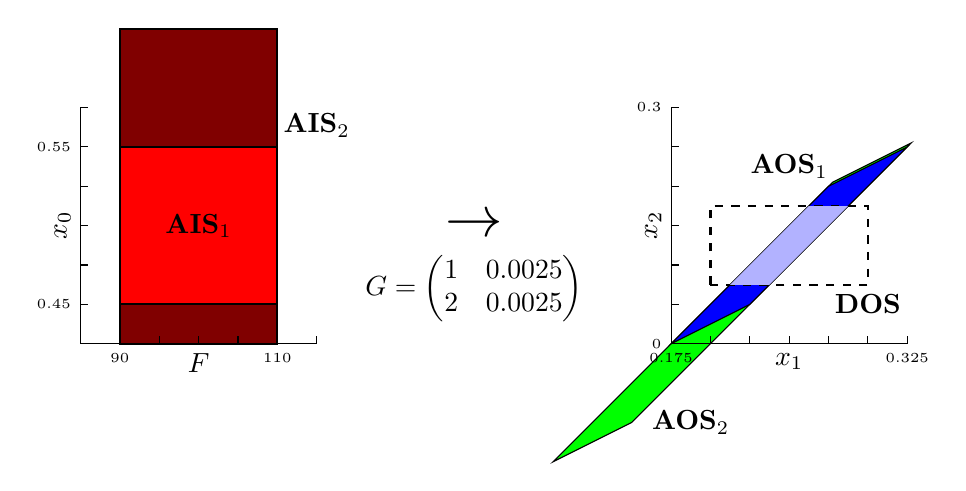
\begin{tikzpicture}[scale=1,stream/.style={->,thick}]
    %AIS
    \draw [thick,fill=red!50!black] (0.5,0) rectangle (2.5,4);
    \node [above] at (3,2.5){\bf AIS$_2$};
    \draw (0,0) -- coordinate (x axis mid) (3,0);
    \draw (0,0) -- coordinate (y axis mid) (0,3);
    \foreach \x in {0,0.5,...,3}
      \draw (\x,0) -- (\x,0.1);
    \foreach \y in {0,0.5,...,3}
      \draw (0,\y) -- (0.1,\y);
    \node[below] at (x axis mid) {$F$};
    \node[below] at (0.5,0) {\tiny 90};
    \node[below] at (2.5,0) {\tiny 110};
    \node[rotate=90, above] at (y axis mid) {$x_0$};
    \node[left] at (0,0.5) {\tiny 0.45};
    \node[left] at (0,2.5) {\tiny 0.55};
    \draw [thick,fill=red] (0.5,0.5) rectangle (2.5,2.5);
    \node at (1.5,1.5){\bf AIS$_1$};
    
    \node at (5,1.5){\bf \huge $\to$};
    \node [below] at (5,1.25){$G=\bpm 1 & 0.0025 \\
                               2 & 0.0025 \epm$};
    
    %AOS
    \def\mx{20}; \def\px{4};
    \def\my{10};

    \draw [fill=green]      (0.2775*\mx + \px, 0.205*\my) 
                         -- (0.3275*\mx + \px, 0.255*\my) 
                         -- (0.15*\mx + \px, -0.1*\my) 
                         -- (0.1*\mx + \px, -0.15*\my) -- cycle;
    \node at (7.75,-1){\bf AOS$_2$};

    \draw (7.5,0) -- coordinate (x axis mid) (3+7.5,0);
    \draw (7.5,0) -- coordinate (y axis mid) (7.5,3);
    \foreach \x in {7.5,8,...,10.5}
      \draw (\x,0) -- (\x,0.1);
    \foreach \y in {0,0.5,...,3}
      \draw (7.5,\y) -- (7.6,\y);
    \node[below] at (x axis mid) {$x_1$};
    \node[below] at (7.5,0) {\tiny 0.175};
    \node[below] at (10.5,0) {\tiny 0.325};
    \node[rotate=90, above] at (y axis mid) {$x_2$};
    \node[left] at (7.5,0) {\tiny 0};
    \node[left] at (7.5,3) {\tiny 0.3};
    \draw [fill=blue] (0.175*\mx + \px , 0) 
                         -- (0.225*\mx + \px,0.05*\my) 
                         -- (0.325*\mx + \px,0.25*\my) 
                         -- (0.275*\mx + \px,0.2*\my) -- cycle;
    \node at (9,2.25){\bf AOS$_1$};    
    % DOS  0.25 0.125
    \draw [thick,dashed] (0.2*\mx + \px,0.075*\my) rectangle
                         (0.3*\mx + \px,0.175*\my);
    \node at (10,0.5){\bf DOS};    

    \begin{scope}
    \clip (0.2*\mx + \px,0.075*\my) rectangle
                         (0.3*\mx + \px,0.175*\my);
    \clip (0.175*\mx + \px , 0) 
                         -- (0.225*\mx + \px,0.05*\my) 
                         -- (0.325*\mx + \px,0.25*\my) 
                         -- (0.275*\mx + \px,0.2*\my) -- cycle;
    \fill[color=blue!30] (0.2*\mx + \px,0.075*\my) rectangle
                         (0.3*\mx + \px,0.175*\my);
    \end{scope}    

  \end{tikzpicture}
\end{center}
\end{frame}


\begin{frame}{Reformatting Constraints for Use with Commercial MPCs}
Most commercial MPCs allow only high/low limits.
\vfill
Constraints can be handled in the same way unmeasured variables are added;
  \begin{itemize}
    \item
      Common technique in industry
    \item
      Linear combinations of other variables
    \item
      Linear inequality can be expressed as high/low limits
    \item
      Increases dimensionality of problem
  \end{itemize}
\vfill
\end{frame}

\subsection{Constraint Set Fitting}

\begin{frame}{The Purpose of Fitting Constraint Sets}
Constraint set fitting can be advantageous;
  \begin{itemize}
    \item
      Decrease the control problem
    \item
      Conform to commercial MPC structure
    \item
      Calculate actual/realistic controlability
  \end{itemize}
\end{frame}

\begin{frame}{Formulating the Problem}
Fit the largest volume polytope inside the initial constraint set.
\vfill
Subject to;
  \begin{itemize}
    \item
      Polytope inside initial set
    \item
      Polytope must be convex
    \item
      Specified number of faces on polytope
  \end{itemize}
\vfill
\end{frame}

\begin{frame}{Different Problem Formulations}
\begin{wrapfigure}{r}{45mm}
  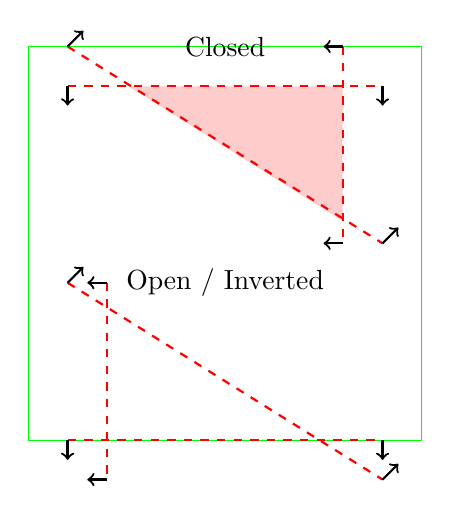
\begin{tikzpicture}[scale=1,stream/.style={->,thick}]
    \draw [color=green] (0,3) rectangle (5,-2);
    
    \draw [color=white,fill=red!20] (4,2.5) -- (4,0.77) -- (1.25,2.5) -- cycle;
    \draw [thick,dashed,color=red] (0.5,2.5) -- (4.5,2.5);
    \draw [thick,dashed,color=red] (4,3) -- (4,0.5);
    \draw [thick,dashed,color=red] (0.5,3) -- (4.5,0.5);
    \draw [thick,<-] (0.5,2.25)--(0.5,2.5);
    \draw [thick,->] (4.5,2.5)--(4.5,2.25);
    \draw [thick,->] (4,3) -- (3.75,3);
    \draw [thick,->] (4,0.5) -- (3.75,0.5);
    \draw [thick,->] (0.5,3) -- (0.7,3.2);
    \draw [thick,->] (4.5,0.5) -- (4.7,0.7);
    \node at (2.5,3){Closed};
    
    \def\py{-3};
    \draw [thick,dashed,color=red] (0.5,2.5-4.5) -- (4.5,2.5-4.5);
    \draw [thick,dashed,color=red] (1,3-3) -- (1,0.5-3);
    \draw [thick,dashed,color=red] (0.5,3+\py) -- (4.5,0.5+\py);
    \draw [thick,<-] (0.5,2.25-4.5)--(0.5,2.5-4.5);
    \draw [thick,->] (4.5,2.5-4.5)--(4.5,2.25-4.5);
    \draw [thick,->] (4-3,3-3) -- (3.75-3,3-3);
    \draw [thick,->] (4-3,0.5-3) -- (3.75-3,0.5-3);
    \draw [thick,->] (0.5,3+\py) -- (0.7,3.2+\py);
    \draw [thick,->] (4.5,0.5+\py) -- (4.7,0.7+\py);
    \node at (2.5,0){Open / Inverted};

  \end{tikzpicture}
\end{wrapfigure}
Faces vs Vertices; which is better?
\vfill
Using a face-based formulation:
\begin{itemize}
  \item
    Pros;
      \begin{itemize}
        \item
          Fixed face number
        \item
          More rigorous approach
      \end{itemize}
  \item
    Cons;
      \begin{itemize}
        \item
          Inconsistent gradient\\ information
        \item
          Superfluous degrees \\of freedom
        \item
          Shape inversion
      \end{itemize}
\end{itemize}
\vfill
\end{frame}

\begin{frame}{Different Problem Formulations (cont.)}
\begin{wrapfigure}{r}{45mm}
  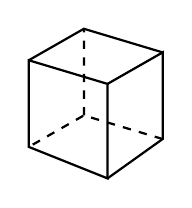
\begin{tikzpicture}[scale=0.1,stream/.style={->,thick}]
    %cube
    \draw [thick] (0,0) -- (0,12) -- (-10,15) -- (-10,4) -- cycle; 
    \draw [thick] (0,0) -- (7,5) -- (7,16) -- (0,12); 
    \draw [thick] (7,16) -- (-3,19) -- (-10,15); 
    \draw [thick,dashed] (7,5) -- (-3,8) -- (-10,4) (-3,8) -- (-3,19); 
  \end{tikzpicture}
  \quad
  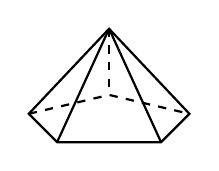
\begin{tikzpicture}[scale=0.06,stream/.style={->,thick}]
    %pentagonal pyramid  
    \draw [thick] (-6,6) -- (0,0) -- (22,0) -- (28,6) -- (11,24) -- cycle; 
    \draw [thick] (11,24) -- (0,0); 
    \draw [thick] (11,24) -- (22,0); 
    \draw [thick,dashed] (-6,6) -- (11,10) -- (28,6); 
    \draw [thick,dashed] (11,24) -- (11,10); 
  \end{tikzpicture}
  \vfill
  \begin{center}
    \scalebox{0.5}{% Graphic for TeX using PGF
% Title: /home/andre/Diagram1.dia
% Creator: Dia v0.97.1
% CreationDate: Fri Oct 15 16:59:06 2010
% For: andre
% \usepackage{tikz}
% The following commands are not supported in PSTricks at present
% We define them conditionally, so when they are implemented,
% this pgf file will use them.
\ifx\du\undefined
  \newlength{\du}
\fi
\setlength{\du}{15\unitlength}
\begin{tikzpicture}
\pgftransformxscale{1.000000}
\pgftransformyscale{-1.000000}
\definecolor{dialinecolor}{rgb}{0.000000, 0.000000, 0.000000}
\pgfsetstrokecolor{dialinecolor}
\definecolor{dialinecolor}{rgb}{1.000000, 1.000000, 1.000000}
\pgfsetfillcolor{dialinecolor}
\pgfsetlinewidth{0.100000\du}
\pgfsetdash{}{0pt}
\pgfsetdash{}{0pt}
\pgfsetmiterjoin
\pgfsetbuttcap
\definecolor{dialinecolor}{rgb}{1.000000, 1.000000, 1.000000}
\pgfsetfillcolor{dialinecolor}
\fill (-11.693750\du,1.831039\du)--(-6.193750\du,1.081039\du)--(-2.943750\du,4.981039\du)--(-4.643750\du,9.431039\du)--(-10.193750\du,9.081039\du)--cycle;
\definecolor{dialinecolor}{rgb}{0.000000, 0.000000, 0.000000}
\pgfsetstrokecolor{dialinecolor}
\draw (-11.693750\du,1.831039\du)--(-6.193750\du,1.081039\du)--(-2.943750\du,4.981039\du)--(-4.643750\du,9.431039\du)--(-10.193750\du,9.081039\du)--cycle;
\pgfsetlinewidth{0.100000\du}
\pgfsetdash{}{0pt}
\pgfsetdash{}{0pt}
\pgfsetbuttcap
\pgfsetmiterjoin
\pgfsetlinewidth{0.100000\du}
\pgfsetbuttcap
\pgfsetmiterjoin
\pgfsetdash{}{0pt}
\definecolor{dialinecolor}{rgb}{1.000000, 0.000000, 0.000000}
\pgfsetfillcolor{dialinecolor}
\pgfpathellipse{\pgfpoint{-2.956250\du}{5.049789\du}}{\pgfpoint{0.306250\du}{0\du}}{\pgfpoint{0\du}{0.306250\du}}
\pgfusepath{fill}
\definecolor{dialinecolor}{rgb}{1.000000, 0.000000, 0.000000}
\pgfsetstrokecolor{dialinecolor}
\pgfpathellipse{\pgfpoint{-2.956250\du}{5.049789\du}}{\pgfpoint{0.306250\du}{0\du}}{\pgfpoint{0\du}{0.306250\du}}
\pgfusepath{stroke}
\pgfsetbuttcap
\pgfsetmiterjoin
\pgfsetdash{}{0pt}
\definecolor{dialinecolor}{rgb}{1.000000, 0.000000, 0.000000}
\pgfsetstrokecolor{dialinecolor}
\pgfpathellipse{\pgfpoint{-2.956250\du}{5.049789\du}}{\pgfpoint{0.306250\du}{0\du}}{\pgfpoint{0\du}{0.306250\du}}
\pgfusepath{stroke}
\pgfsetlinewidth{0.100000\du}
\pgfsetdash{}{0pt}
\pgfsetdash{}{0pt}
\pgfsetbuttcap
\pgfsetmiterjoin
\pgfsetlinewidth{0.100000\du}
\pgfsetbuttcap
\pgfsetmiterjoin
\pgfsetdash{}{0pt}
\definecolor{dialinecolor}{rgb}{1.000000, 0.000000, 0.000000}
\pgfsetfillcolor{dialinecolor}
\pgfpathellipse{\pgfpoint{-11.696250\du}{1.852289\du}}{\pgfpoint{0.306250\du}{0\du}}{\pgfpoint{0\du}{0.306250\du}}
\pgfusepath{fill}
\definecolor{dialinecolor}{rgb}{1.000000, 0.000000, 0.000000}
\pgfsetstrokecolor{dialinecolor}
\pgfpathellipse{\pgfpoint{-11.696250\du}{1.852289\du}}{\pgfpoint{0.306250\du}{0\du}}{\pgfpoint{0\du}{0.306250\du}}
\pgfusepath{stroke}
\pgfsetbuttcap
\pgfsetmiterjoin
\pgfsetdash{}{0pt}
\definecolor{dialinecolor}{rgb}{1.000000, 0.000000, 0.000000}
\pgfsetstrokecolor{dialinecolor}
\pgfpathellipse{\pgfpoint{-11.696250\du}{1.852289\du}}{\pgfpoint{0.306250\du}{0\du}}{\pgfpoint{0\du}{0.306250\du}}
\pgfusepath{stroke}
\pgfsetlinewidth{0.100000\du}
\pgfsetdash{}{0pt}
\pgfsetdash{}{0pt}
\pgfsetbuttcap
\pgfsetmiterjoin
\pgfsetlinewidth{0.100000\du}
\pgfsetbuttcap
\pgfsetmiterjoin
\pgfsetdash{}{0pt}
\definecolor{dialinecolor}{rgb}{1.000000, 0.000000, 0.000000}
\pgfsetfillcolor{dialinecolor}
\pgfpathellipse{\pgfpoint{-6.223750\du}{1.104789\du}}{\pgfpoint{0.306250\du}{0\du}}{\pgfpoint{0\du}{0.306250\du}}
\pgfusepath{fill}
\definecolor{dialinecolor}{rgb}{1.000000, 0.000000, 0.000000}
\pgfsetstrokecolor{dialinecolor}
\pgfpathellipse{\pgfpoint{-6.223750\du}{1.104789\du}}{\pgfpoint{0.306250\du}{0\du}}{\pgfpoint{0\du}{0.306250\du}}
\pgfusepath{stroke}
\pgfsetbuttcap
\pgfsetmiterjoin
\pgfsetdash{}{0pt}
\definecolor{dialinecolor}{rgb}{1.000000, 0.000000, 0.000000}
\pgfsetstrokecolor{dialinecolor}
\pgfpathellipse{\pgfpoint{-6.223750\du}{1.104789\du}}{\pgfpoint{0.306250\du}{0\du}}{\pgfpoint{0\du}{0.306250\du}}
\pgfusepath{stroke}
\pgfsetlinewidth{0.100000\du}
\pgfsetdash{}{0pt}
\pgfsetdash{}{0pt}
\pgfsetbuttcap
\pgfsetmiterjoin
\pgfsetlinewidth{0.100000\du}
\pgfsetbuttcap
\pgfsetmiterjoin
\pgfsetdash{}{0pt}
\definecolor{dialinecolor}{rgb}{1.000000, 0.000000, 0.000000}
\pgfsetfillcolor{dialinecolor}
\pgfpathellipse{\pgfpoint{-10.201250\du}{9.057289\du}}{\pgfpoint{0.306250\du}{0\du}}{\pgfpoint{0\du}{0.306250\du}}
\pgfusepath{fill}
\definecolor{dialinecolor}{rgb}{1.000000, 0.000000, 0.000000}
\pgfsetstrokecolor{dialinecolor}
\pgfpathellipse{\pgfpoint{-10.201250\du}{9.057289\du}}{\pgfpoint{0.306250\du}{0\du}}{\pgfpoint{0\du}{0.306250\du}}
\pgfusepath{stroke}
\pgfsetbuttcap
\pgfsetmiterjoin
\pgfsetdash{}{0pt}
\definecolor{dialinecolor}{rgb}{1.000000, 0.000000, 0.000000}
\pgfsetstrokecolor{dialinecolor}
\pgfpathellipse{\pgfpoint{-10.201250\du}{9.057289\du}}{\pgfpoint{0.306250\du}{0\du}}{\pgfpoint{0\du}{0.306250\du}}
\pgfusepath{stroke}
\pgfsetlinewidth{0.100000\du}
\pgfsetdash{}{0pt}
\pgfsetdash{}{0pt}
\pgfsetbuttcap
\pgfsetmiterjoin
\pgfsetlinewidth{0.100000\du}
\pgfsetbuttcap
\pgfsetmiterjoin
\pgfsetdash{}{0pt}
\definecolor{dialinecolor}{rgb}{1.000000, 0.000000, 0.000000}
\pgfsetfillcolor{dialinecolor}
\pgfpathellipse{\pgfpoint{-4.678750\du}{9.459789\du}}{\pgfpoint{0.306250\du}{0\du}}{\pgfpoint{0\du}{0.306250\du}}
\pgfusepath{fill}
\definecolor{dialinecolor}{rgb}{1.000000, 0.000000, 0.000000}
\pgfsetstrokecolor{dialinecolor}
\pgfpathellipse{\pgfpoint{-4.678750\du}{9.459789\du}}{\pgfpoint{0.306250\du}{0\du}}{\pgfpoint{0\du}{0.306250\du}}
\pgfusepath{stroke}
\pgfsetbuttcap
\pgfsetmiterjoin
\pgfsetdash{}{0pt}
\definecolor{dialinecolor}{rgb}{1.000000, 0.000000, 0.000000}
\pgfsetstrokecolor{dialinecolor}
\pgfpathellipse{\pgfpoint{-4.678750\du}{9.459789\du}}{\pgfpoint{0.306250\du}{0\du}}{\pgfpoint{0\du}{0.306250\du}}
\pgfusepath{stroke}
\pgfsetlinewidth{0.100000\du}
\pgfsetdash{}{0pt}
\pgfsetdash{}{0pt}
\pgfsetbuttcap
\pgfsetmiterjoin
\pgfsetlinewidth{0.100000\du}
\pgfsetbuttcap
\pgfsetmiterjoin
\pgfsetdash{}{0pt}
\definecolor{dialinecolor}{rgb}{1.000000, 0.000000, 0.000000}
\pgfsetfillcolor{dialinecolor}
\pgfpathellipse{\pgfpoint{-9.006250\du}{4.887289\du}}{\pgfpoint{0.306250\du}{0\du}}{\pgfpoint{0\du}{0.306250\du}}
\pgfusepath{fill}
\definecolor{dialinecolor}{rgb}{1.000000, 0.000000, 0.000000}
\pgfsetstrokecolor{dialinecolor}
\pgfpathellipse{\pgfpoint{-9.006250\du}{4.887289\du}}{\pgfpoint{0.306250\du}{0\du}}{\pgfpoint{0\du}{0.306250\du}}
\pgfusepath{stroke}
\pgfsetbuttcap
\pgfsetmiterjoin
\pgfsetdash{}{0pt}
\definecolor{dialinecolor}{rgb}{1.000000, 0.000000, 0.000000}
\pgfsetstrokecolor{dialinecolor}
\pgfpathellipse{\pgfpoint{-9.006250\du}{4.887289\du}}{\pgfpoint{0.306250\du}{0\du}}{\pgfpoint{0\du}{0.306250\du}}
\pgfusepath{stroke}
\pgfsetlinewidth{0.100000\du}
\pgfsetdash{}{0pt}
\pgfsetdash{}{0pt}
\pgfsetbuttcap
\pgfsetmiterjoin
\pgfsetlinewidth{0.100000\du}
\pgfsetbuttcap
\pgfsetmiterjoin
\pgfsetdash{}{0pt}
\definecolor{dialinecolor}{rgb}{1.000000, 0.000000, 0.000000}
\pgfsetfillcolor{dialinecolor}
\pgfpathellipse{\pgfpoint{-6.908750\du}{6.889789\du}}{\pgfpoint{0.306250\du}{0\du}}{\pgfpoint{0\du}{0.306250\du}}
\pgfusepath{fill}
\definecolor{dialinecolor}{rgb}{1.000000, 0.000000, 0.000000}
\pgfsetstrokecolor{dialinecolor}
\pgfpathellipse{\pgfpoint{-6.908750\du}{6.889789\du}}{\pgfpoint{0.306250\du}{0\du}}{\pgfpoint{0\du}{0.306250\du}}
\pgfusepath{stroke}
\pgfsetbuttcap
\pgfsetmiterjoin
\pgfsetdash{}{0pt}
\definecolor{dialinecolor}{rgb}{1.000000, 0.000000, 0.000000}
\pgfsetstrokecolor{dialinecolor}
\pgfpathellipse{\pgfpoint{-6.908750\du}{6.889789\du}}{\pgfpoint{0.306250\du}{0\du}}{\pgfpoint{0\du}{0.306250\du}}
\pgfusepath{stroke}
\pgfsetlinewidth{0.100000\du}
\pgfsetdash{}{0pt}
\pgfsetdash{}{0pt}
\pgfsetbuttcap
\pgfsetmiterjoin
\pgfsetlinewidth{0.100000\du}
\pgfsetbuttcap
\pgfsetmiterjoin
\pgfsetdash{}{0pt}
\definecolor{dialinecolor}{rgb}{1.000000, 0.000000, 0.000000}
\pgfsetfillcolor{dialinecolor}
\pgfpathellipse{\pgfpoint{-5.361250\du}{3.342289\du}}{\pgfpoint{0.306250\du}{0\du}}{\pgfpoint{0\du}{0.306250\du}}
\pgfusepath{fill}
\definecolor{dialinecolor}{rgb}{1.000000, 0.000000, 0.000000}
\pgfsetstrokecolor{dialinecolor}
\pgfpathellipse{\pgfpoint{-5.361250\du}{3.342289\du}}{\pgfpoint{0.306250\du}{0\du}}{\pgfpoint{0\du}{0.306250\du}}
\pgfusepath{stroke}
\pgfsetbuttcap
\pgfsetmiterjoin
\pgfsetdash{}{0pt}
\definecolor{dialinecolor}{rgb}{1.000000, 0.000000, 0.000000}
\pgfsetstrokecolor{dialinecolor}
\pgfpathellipse{\pgfpoint{-5.361250\du}{3.342289\du}}{\pgfpoint{0.306250\du}{0\du}}{\pgfpoint{0\du}{0.306250\du}}
\pgfusepath{stroke}
\end{tikzpicture}
}
  \end{center}
\end{wrapfigure}
Using a vertex-based formulation:
\begin{itemize}
  \item
    Pros;
    \begin{itemize}
      \item
        Direct constraint checking
      \item
        Consistent gradient \\information
      \item
        More intuitive approach
    \end{itemize}
  \item
    Cons;
    \begin{itemize}
      \item
        Variable number
      \item
        Convexity checks
      \item
        Number of faces problems
    \end{itemize}
\end{itemize}
\vfill
\end{frame}

\begin{frame}{Setting Up Objective Functions}
Positive and negative volumes
\begin{itemize}
  \item
    Shape inversion
  \item
    Shape exceptions
\end{itemize}
\vfill
Scaling of the problem;
\begin{itemize}
  \item
    $f({\bf x}) = f(n{\bf x})$
  \item
    Using up degrees of freedom
\end{itemize}
\vfill
\end{frame}

\begin{frame}{Setting Up Objective Functions (cont.)}
% cube vs arb
% comp effort
Dependant on optimizer/solver used;
\begin{itemize}
  \item
    Unconstrained solver
    \begin{itemize}
      \item
        Downhill-Simplex
      \item
        Penalty formulation
    \end{itemize}
  \item
    Constrained solver
    \begin{itemize}
      \item
        SLSQP (Gradient based)
      \item
        Equality / Inequality constraints
    \end{itemize}
\end{itemize}
\end{frame}


\begin{frame}{Solving the Problem (Fitting the Set)}
Starting point generation
\vfill
Solution times;
\begin{itemize}
  \item
    Downhill-Simplex
  \item
    SLSQP
\end{itemize}
\vfill
\end{frame}

\begin{frame}{Some Fitting Results}
[insert fitting results]
\end{frame}


\section{Practical Application}

\subsection{Laboratory Distillation Column}

\begin{frame}{A Simplified Distillation Model}
\scalebox{0.15}{\includegraphics{Pmc05distil_rig}}
\end{frame}

\begin{frame}{Constraint Information and Results}
[apply method to model,\\
show some results/graphs]
\end{frame}

\begin{frame}{Interfacing with Honeywell's RMPCT}
\scalebox{0.32}{\includegraphics{CV1}}
\end{frame}


\section*{Summary}

\begin{frame}{Summary}

  % Keep the summary *very short*.
  \begin{itemize}
  \item
    MPC is a popular control algorithm but rigorous constraint handling and
    understanding are lacking.
  \item
    The proposed framework disambiguates the language used and allows for
    \begin{itemize}
      \item
        fitting of constraint sets,
      \item
        checking constraint feasibility and
      \item
        reformatting constraints for use in commercial packages.
    \end{itemize}
  \end{itemize}
 
\end{frame}



% All of the following is optional and typically not needed. 
\appendix
\section<presentation>*{\appendixname}
\subsection<presentation>*{For Further Reading}

\begin{frame}
  \frametitle<presentation>{For Further Reading}
    
  \begin{thebibliography}{10}
    
  \beamertemplatebookbibitems
  % Start with overview books.

  \bibitem{Rawlings2009}
    JB. Rawlings and DQ. Mayne
    \newblock {\em Model Predictive Control: Theory and Design}.
    \newblock Nob Hill Publishing, 2009.
 
    
  \beamertemplatearticlebibitems
  % Followed by interesting articles. Keep the list short. 

  \bibitem{Vinson2000}
    DR. Vinson and C. Georgakis
    \newblock A New Measure for Process Output Controlability
    \newblock {\em Journal of Process Control}, 10:185--194,
    2000.
  
  \bibitem{Lima2008}
    FV. Lima and C. Georgakis
    \newblock Design of Output Constraints for Model-based
      Non-Square Controllers Using Interval Operability
    \newblock {\em Journal of Process Control}, 18:610--620,
    2008.
  
\end{thebibliography}
\end{frame}

\end{document}


